\documentclass{beamer}

\usepackage[utf8]{inputenc}
\usepackage[T1]{fontenc}
\usepackage[francais]{babel}
\usepackage{hyperref}
\usetheme{Madrid}

\makeatletter
\setbeamertemplate{footline}{
  \leavevmode%
  \hbox{%
  \begin{beamercolorbox}[wd=.2\paperwidth,ht=2.25ex,dp=1ex,center]{author in head/foot}%
    \usebeamerfont{author in head/foot}\insertshortauthor
  \end{beamercolorbox}%
  \begin{beamercolorbox}[wd=.55\paperwidth,ht=2.25ex,dp=1ex,center]{title in head/foot}%
    \usebeamerfont{title in head/foot}Soutenance TER
  \end{beamercolorbox}%
  \begin{beamercolorbox}[wd=.25\paperwidth,ht=2.25ex,dp=1ex,right]{date in head/foot}%
    \usebeamerfont{date in head/foot}\insertshortdate{}\hspace*{2em}
    \insertframenumber{} / \inserttotalframenumber\hspace*{2ex} 
  \end{beamercolorbox}}%
  \vskip0pt%
}
\makeatother
\title{Analyse et amélioration des performances d'un programme par compilation optimisante: Étude de cas}

\subtitle{TER M1 Informatique}

\author[Pierre \textsc{Tassel}]{Pierre \textsc{Tassel} sous la direction du Pr \textsc{Touati}}

\institute[Universitée Nice Sophia Antipolis] 
{Département Informatique\\
Universitée Nice Sophia Antipolis
\and
Master Informatique}

\date{\today}

\subject{Présentation TER}

% Let's get started
\begin{document}
%\author{Pierre \textsc{Tassel}}
\begin{frame}
  \titlepage
\end{frame}

\begin{frame}{Plan}
  \tableofcontents
  % You might wish to add the option [pausesections]
\end{frame}

% Section and subsections will appear in the presentation overview
% and table of contents.
\section{Présentation du programme}

\begin{frame}{Présentation du programme}{MinMax et le jeux de l'Awale}
\begin{itemize}
  \item
    MinMax avec coupes Alpha Bêta.
  \item
    Variante du jeux de l'Awale avec 6 cases et 4 graines par case.
  \item
    Ecrit en C++ par Pr \textsc{Régin}.
  \end{itemize}
  \begin{figure}
   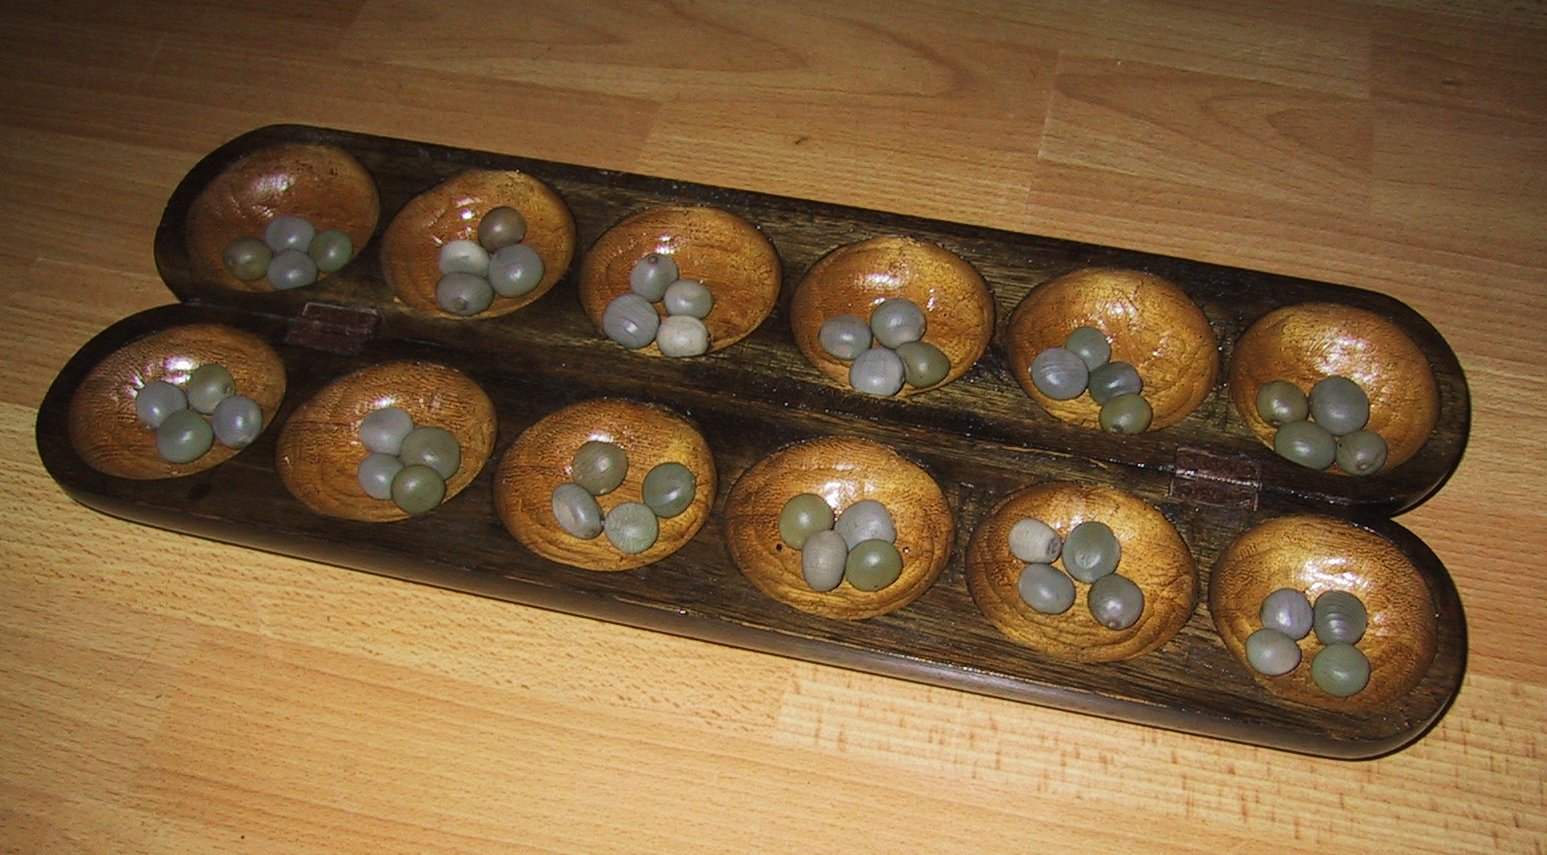
\includegraphics[width= 0.7\linewidth, keepaspectratio]{Awale.jpg}
   \caption{Le jeu de l'Awalé.\label{Fig:awale}}
\end{figure}
\end{frame}

\section{Démarche expérimentale}
\begin{frame}{Démarche expérimentale}{Environnement matériel et logiciel}
\begin{itemize}
  \item
  	\textit{Processeur Scaling} désactivé, processeur Intel core i7 8 coeurs 2,5GHz, 8Go DDR3, 256Go de SSD.
  \item
    Environnement minimaliste en CLI, Arch Linux basé sur le noyau Linux 4.14.13-1.
    \item
    Trois compilateurs analysés\,: GCC, ICC et CLang (dernières versions disponible).
    \item
    Fichier d'entrée généré en faisant jouer le programme contre lui même, programme déterministe.
    \item
    Les exécutions sont répétés 20 fois pour chaque configuration testée.
\end{itemize}
\end{frame}

\section{Analyse et optimisation des performances séquentielles}

\begin{frame}{Analyse des performances séquentielles}

\begin{figure}
      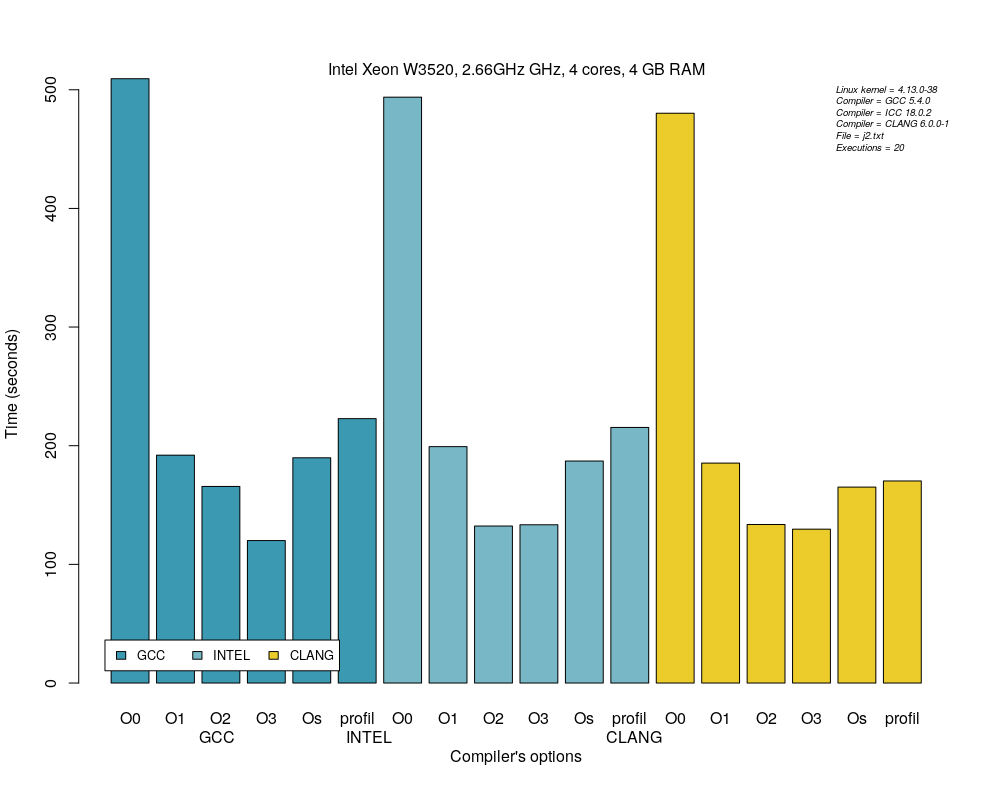
\includegraphics[width=0.7\textwidth]{GCCvsICCvsCLANG_j2.png}
      \caption{Temps d’exécution séquentiel quand le programme commence.}
\end{figure}
\end{frame}

\begin{frame}{Profilage du code}{GProf}
\begin{figure}
        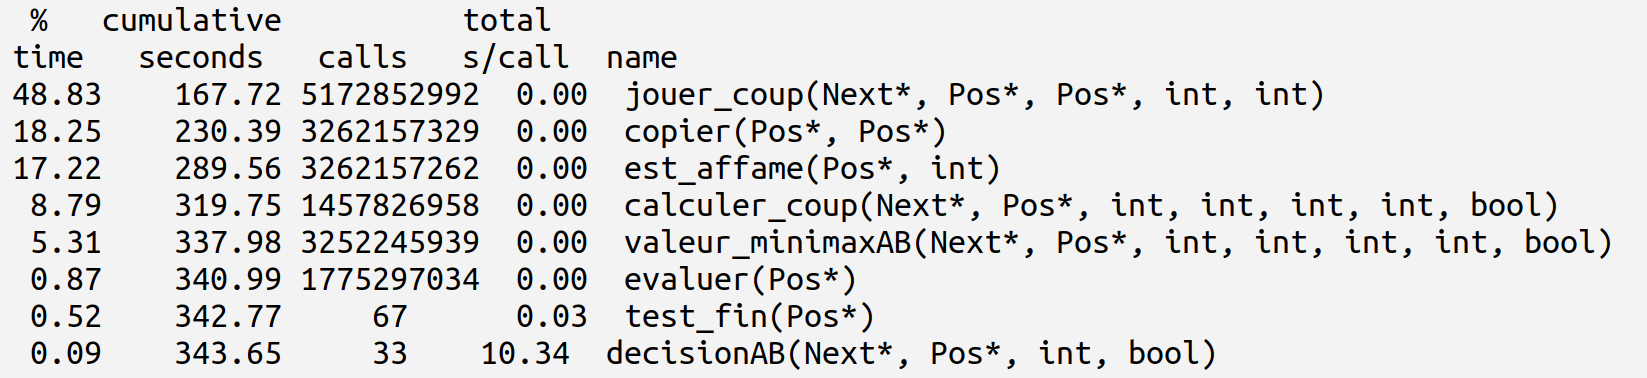
\includegraphics[width=\textwidth]{gprof.png}
        \caption{Profilage du code avec GProf.\label{Fig:GProf}}
\end{figure}
\end{frame}

\begin{frame}{Profilage du code}{vTune}
\begin{columns}
    \column{6.5cm}
    \begin{figure}
      \centering
   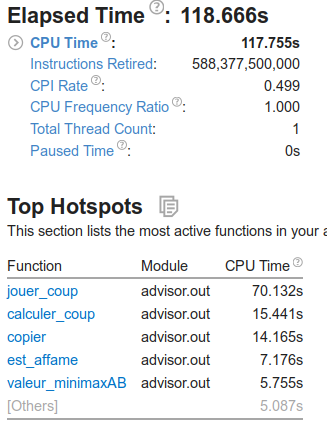
\includegraphics[width=0.75\textwidth]{vtune.png}
   \caption{vTune analyse usage processeur.\label{Fig:vTune_proc}}
    \end{figure}
    \column{6.5cm}
    \begin{figure}
      \centering
   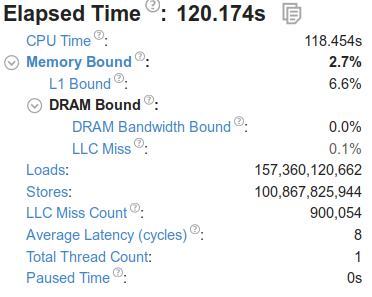
\includegraphics[width=0.9\textwidth]{memory_vtune.png}
   \caption{vTune analyse usage mémoire.\label{Fig:vTune_mem}}
    \end{figure}
    
  \end{columns}
\end{frame}

\section{Ajout de parallélisme}

\begin{frame}{Approche naïve d'ajout de parallélisme}
	\begin{figure}
      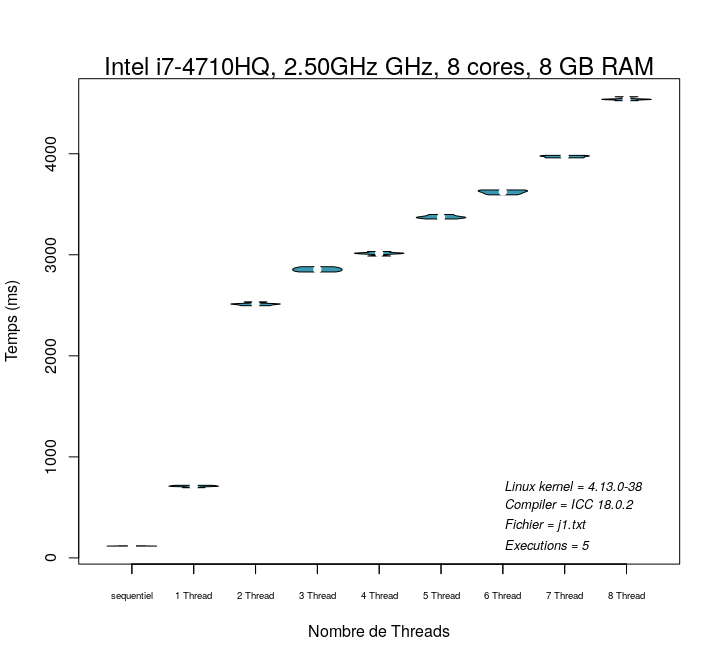
\includegraphics[width=0.7\textwidth]{intel_parallel_naif.png}
      \caption{Résultat ajout parallélisme avec compilateur Intel.\label{Fig:naif_intel}}
  
	\end{figure}
\end{frame}

\begin{frame}{False Sharing}
	\begin{figure}
	\begin{columns}
      \column{.72\linewidth}
      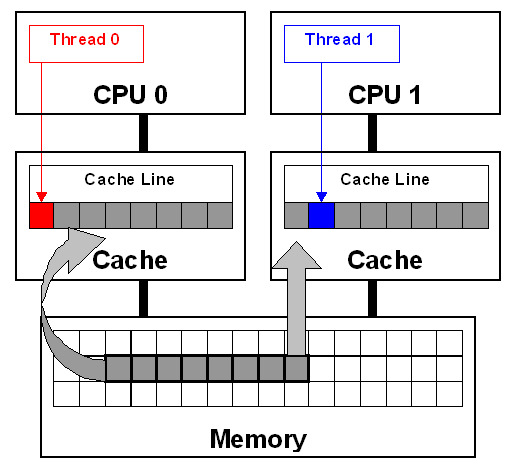
\includegraphics[width=\textwidth]{false_sharing.jpg}
      \column{.25\linewidth}
      \caption{Le phénomène de False Sharing.\label{Fig:false_sharing}}{\href{https://software.intel.com/en-us/articles/avoiding-and-identifying-false-sharing-among-threads}{Source : Documentation Intel.}}
    \end{columns}	
    \end{figure}
\end{frame}

\begin{frame}{Thread Affinity}
	\begin{figure}
	\begin{columns}
      \column{.25\linewidth}
      \caption{Analyse de l'impact du placement des threads avec le compilateur d'Intel, \textbf{-O3} avec 8 CPU.\label{Fig:thread_affinity}}
      \column{.72\linewidth}
      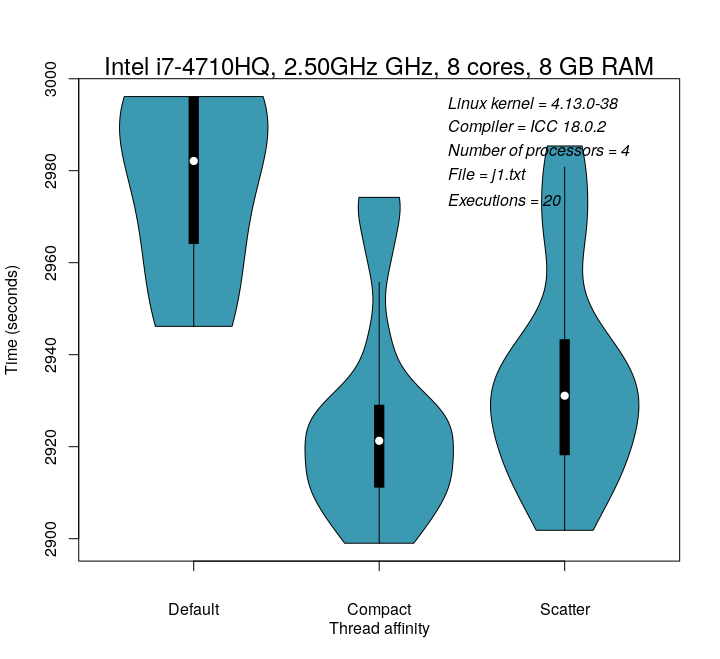
\includegraphics[width=\textwidth]{defaultVSscatterVScompact.png}
    \end{columns}	
	\end{figure}
\end{frame}

\begin{frame}{Intel Advisor}
	\begin{figure}
	\begin{columns}
      \column{.60\linewidth}
      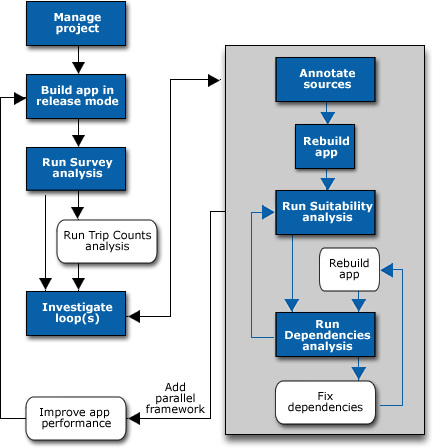
\includegraphics[width=\textwidth]{Intel.jpg}
      \column{.25\linewidth}
      \caption{Méthode itérative pour l'ajout de parallélisme (proposée par Intel).\label{Fig:intel_iter}}{\href{https://software.intel.com/en-us/articles/avoiding-and-identifying-false-sharing-among-threads}{Source : Documentation Intel.}}
    \end{columns}	
    \end{figure}
\end{frame}


\begin{frame}{Difficultés de l'optimisation du code}
\begin{itemize}
\item
Algorithme très séquentiel.
\item
Nombre d'itérations faibles (n = 6).
\item
Usage de pointeurs qui pourraient aveugler les compilateurs.
\end{itemize}
\end{frame}

\section{Modification algorithmique}


\begin{frame}{Modification algorithmique}

\begin{itemize}
  \item
    Trier les coups à évaluer.
  \item
    Table de transposition.
 \end{itemize}	
\end{frame}

\begin{frame}{Trie des coups}
	\begin{figure}
      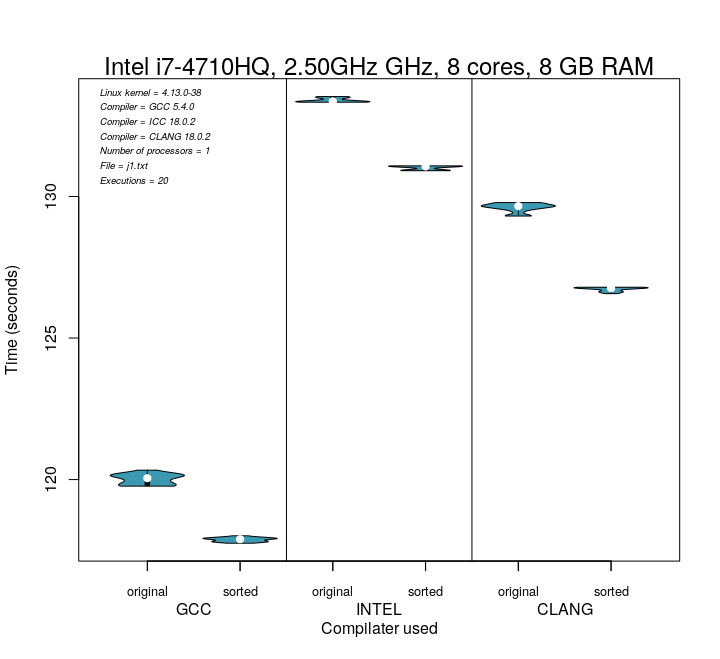
\includegraphics[width=0.7\textwidth]{trie.png}
      \caption{Analyse de l'impact du trie des coups.\label{Fig:trie}}
	\end{figure}
\end{frame}

\begin{frame}{Table de transposition}
	\begin{figure}
	\begin{columns}
      \column{.5\linewidth}
      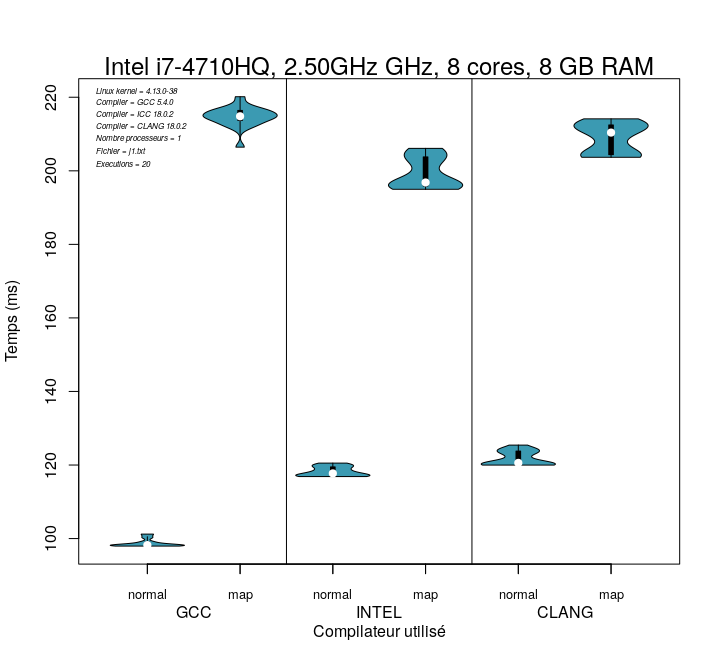
\includegraphics[width=\textwidth]{sorted_map.png}
      \caption{Arbre binaire de recherche.\label{Fig:arbre_binaire}}
      \column{.5\linewidth}
      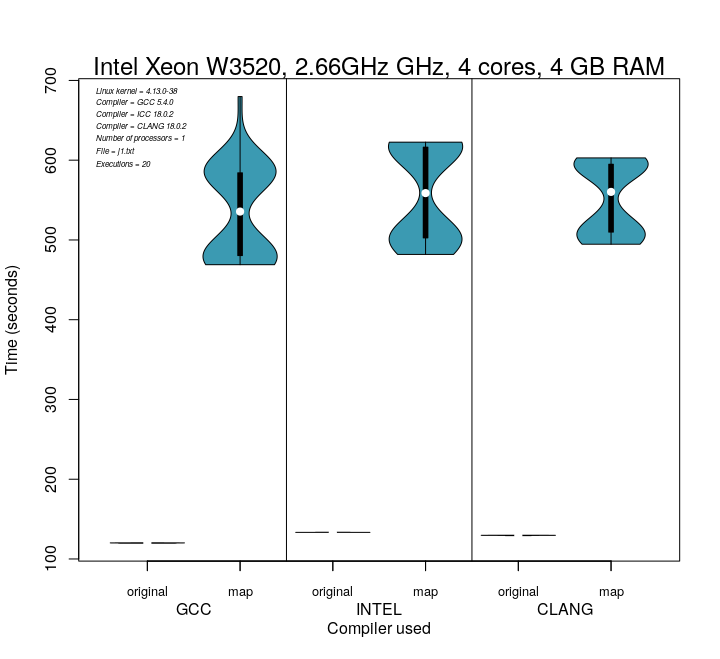
\includegraphics[width=\textwidth]{unsorted_map.png}
      \caption{Table de hashage.\label{Fig:arbre_binaire}}
    \end{columns}	
	\end{figure}
\end{frame}

\section{Conclusion et perspectives}

\begin{frame}{Conclusion et perspectives}
\begin{itemize}
\item
	GCC bat Intel en séquentiel sur architecture Intel.
	\item
	Parallélisation avec OpenMP peut sévèrement dégrader les performances.
  \item
    Phénomène de False Sharing.
  \item
  	Modifications algorithmique nécessaire pour améliorer les performances.
  \item
  	Perspective: Stage à l'\textsc{INRIA}.
 \end{itemize}	
\end{frame}


\end{document}


